\section{The EASY Suites}
This and the following chapter contain an unusual pedagogical tool. It is a combination of a usual example as you find it in most textbooks and a pertinent MATLAB file that does most of the computations where $\sharp$ is between 1 and 18. described in the example. We named the M-files easy$\sharp$ They are published in two parts (suites): Bone presented the first 10 in 2003. The second EASY Suite (number 11 to 18) appears in several issues of the periodical inside GNSS:Borre (2009x), Borre (2009b), Borre (2009c), Borre (2010x), Bone (2010b), and Borre (2010c).
\begin{figure}
	\centering
	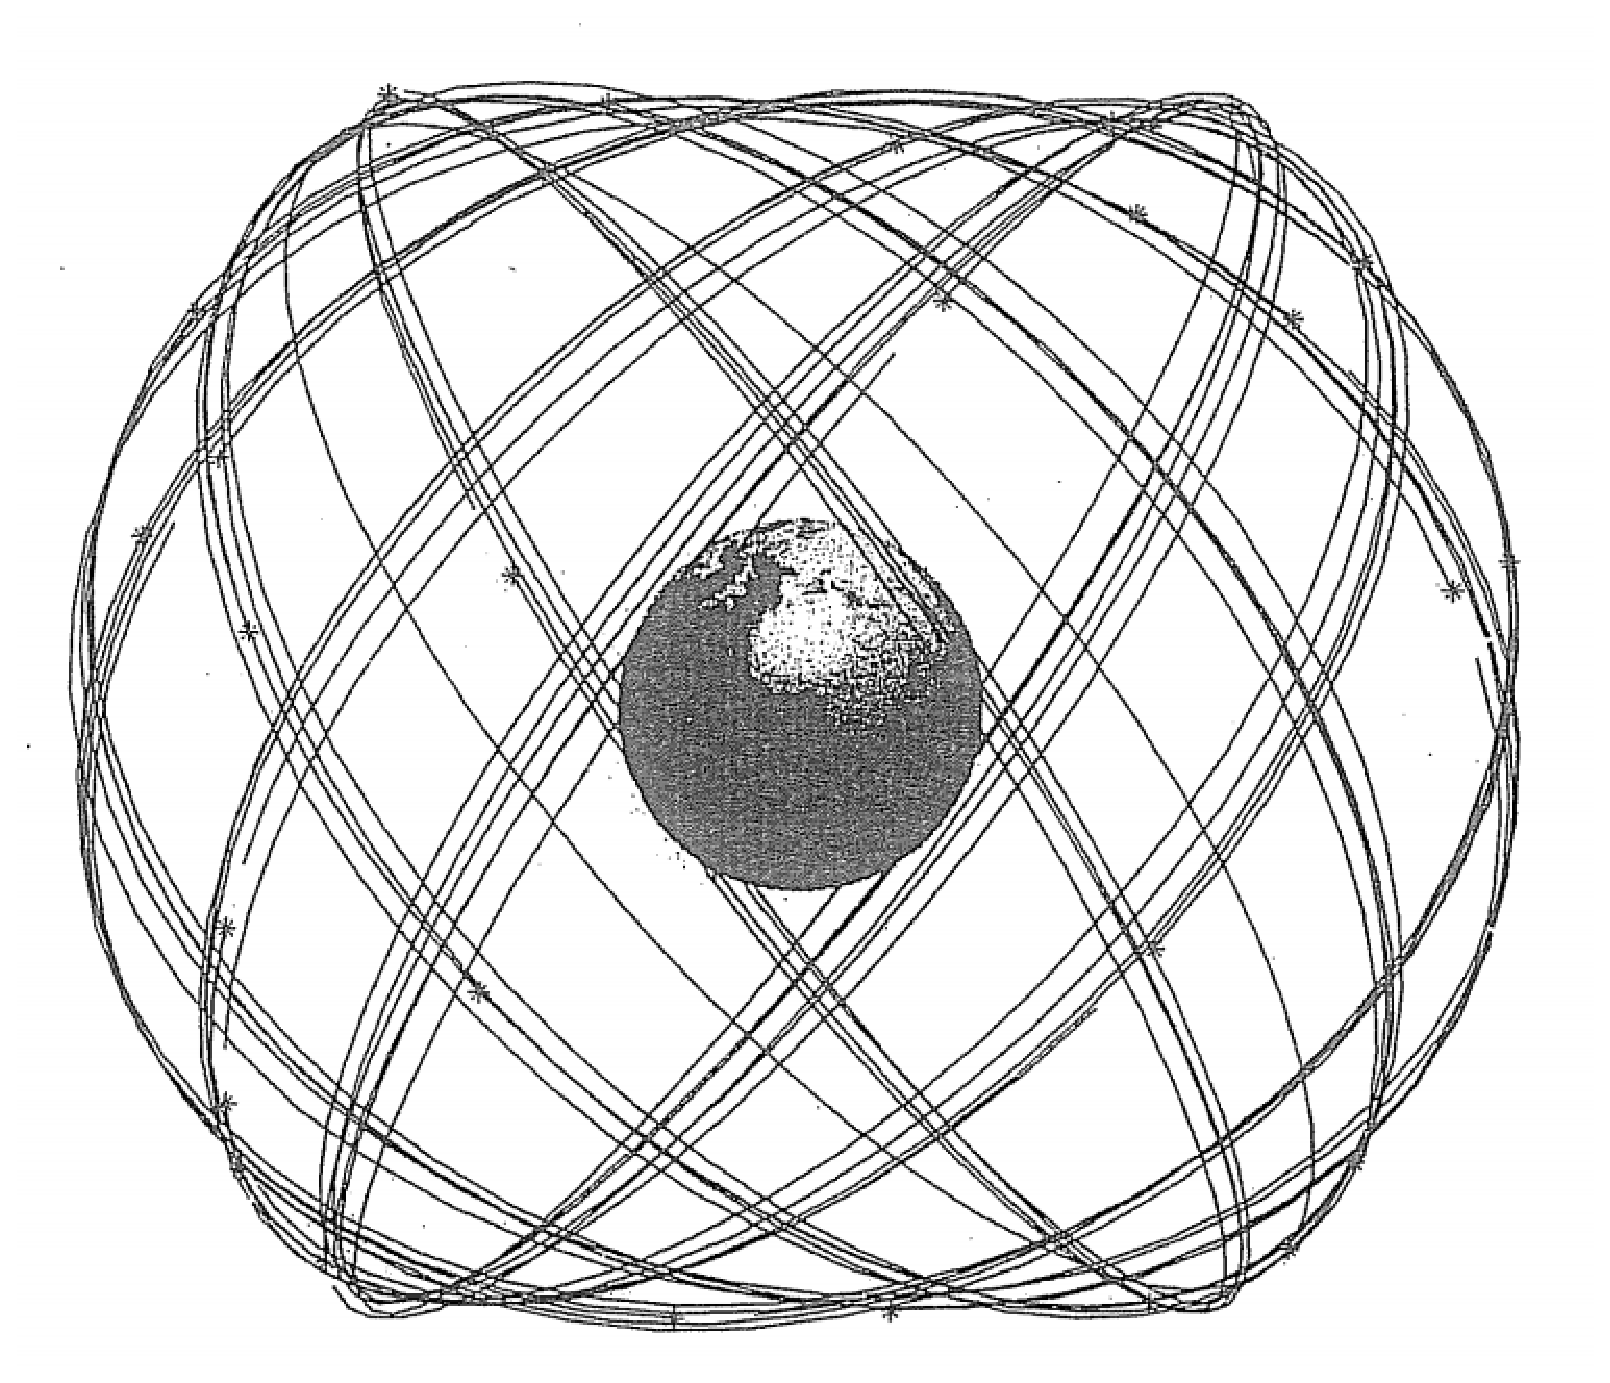
\includegraphics[width=0.4\linewidth]{TeX_files/Part03/chapter09/image/9-1}
	\caption{Satellite orbits in inertial frame— as seen from far out on the line through the intersection between Equator and the Greenwich meridian (latitude $0^\circ$, longitude $0^\circ$). This GPS constellation has 6 planes with 4 satellites. The 2 orbits/day fall 15 minutes short of completion, producing the small gaps at the end of each orbit.}
	\label{fig:9-1}
\end{figure}
\begin{table}
	\caption{Topics Treated in the EASY Suites}
	\footnotesize %设置表格字体大小
	\begin{tabularx}{\textwidth}{cXc}
		\hline  \rule[-2ex]{0pt}{5.5ex}   Name  & 					Topic 						  & Book pages\\ 
		\hline  \rule[-2ex]{0pt}{5.5ex}  easy1  & time conversion: Time, UTC, GPST, week number, and sow  		& \pageref{subsec:easy1} \\ 
		\rule[-2ex]{0pt}{5.5ex}  easy2  & Kepler’s law, computation of a satellite’s position from an ephemeris 			 & \pageref{subsec:easy2}  \\ 
		\rule[-2ex]{0pt}{5.5ex}  easy3  & computation of a receiver’s position in ECEF coordinates from pseudoranges 		 & \pageref{subsec:easy3}  \\ 
		\rule[-2ex]{0pt}{5.5ex}  easy4  & computation of a baseline from pseudoranges alone					   	    & \pageref{subsec:easy4}  \\ 
		\rule[-2ex]{0pt}{5.5ex}  easy5  & computation of a baseline from pseudorange and phase observations using a least-squares solution 	& \pageref{subsec:easy5}\\ 
		\rule[-2ex]{0pt}{5.5ex}  easy6  & the same, but now using a Kalman filter for the baseline estimation	  	   & \pageref{subsec:easy6}  \\ 
		\rule[-2ex]{0pt}{5.5ex}  easy6e & the same as easy5, but introducing downweighting of older observations 			   & \pageref{subsec:easy6e} \\
		\rule[-2ex]{0pt}{5.5ex}  easy7  & estimation of receiver clock offset							& \pageref{subsec:easy7}\\ 
		\rule[-2ex]{0pt}{5.5ex}  easy8  & check of cycle slips and receiver clock reset 						  & \pageref{subsec:easy8}   \\ 
		\rule[-2ex]{0pt}{5.5ex}  easy9  & various coordinate representations of a given baseline							& \pageref{subsec:easy9}   \\ 
		\rule[-2ex]{0pt}{5.5ex}  easy10 & estimation of ionospheric delay for the individual satellites		 		& \pageref{subsec:easy10}   \\ 
		\rule[-2ex]{0pt}{5.5ex}  easy11 & stereographic sky plot of satellite orbits and plot of time when satellites are above a given local horizon & \pageref{subsec:easy11}   \\ 
		\rule[-2ex]{0pt}{5.5ex}  easy12 & details of the LAMBDA method, explained through a small numerical example & \pageref{subsec:easy12}   \\ 
		\rule[-2ex]{0pt}{5.5ex}  easy13 & receiver autonomous integrity monitoring (RAIM), horizontal protection level (HPL), and vertical protection level (VPL) & \pageref{subsec:easy13}   \\ 
		\rule[-2ex]{0pt}{5.5ex}  easy14 & sample of space based augmentation system (SBAS), corrected positions and their presentation in Stanford plots & \pageref{subsec:easy14}   \\ 
		\rule[-2ex]{0pt}{5.5ex}  easy15 & accuracy comparison between pseudorange based stand-alone positions, baselines computed using pseudoranges alone, and combined pseudorange and carrier phase observations & \pageref{subsec:easy15}   \\ 
		\rule[-2ex]{0pt}{5.5ex}  easy16 & error analysis of a selected one-way observation 							& \pageref{subsec:easy16}   \\ 
		\rule[-2ex]{0pt}{5.5ex}  easy17 & satellite orbits in inertial and Earth-centered, Earth-fixed (ECEF) systems, and curve defined by sub-satellite points & \pageref{subsec:easy17}   \\ 
		\rule[-2ex]{0pt}{5.5ex}  easy18 & computation of differential corrections at a base station							 & \pageref{subsec:easy18}   \\ 
		\hline 
	\end{tabularx} 
\end{table}	
The original numbering of those files is maintained. This decision implies that the files in this textbook appear in a seemingly unsorted order. To remedy this fact we include a survey in Table 9.1 on the next page.

The EASY Suites have been created since 2000 to facilitate the understanding of how to code MATLAB for positioning. We start from the basics and build one new topic on top of the earlier files. The topics included in the first EASY Suite were selected to establish a smooth progression in the complexity of the code. The second Suite was written to provide requested code for specialized topics of growing importance. 

The basic data sets we will be working with were collected at Aalborg by two JPS Eurocard receivers on 4 September 2001. The resulting Receiver Independent Exchange (RINEX) files, Gurtner (2000), are site247j.010, site24一1.010, site247j.01 n. For the more specialized topics we need a longer observation series; this is contained in kof r 1.010. 

All the above mentioned files are zipped and made available via the world wide web at $http://gps.aau.dk/\sim borre/easy/$ and $http://gps.aau.dk/\sim borre/easy2/$

	\subsection{Orbits of the Satellites}
	The satellites stay at an altitude of approximately 3 Earth radii.  They travel in nearly circular orbits, two complete orbits in each sidereal day. In practice a pseudorange is most reliable when the satellite is at least $10^\circ$ or better $15^\circ$ above the horizon. Figure 9.1 shows

	\subsection{easy17}\label{subsec:easy17}
	\begin{figure}
		\centering
		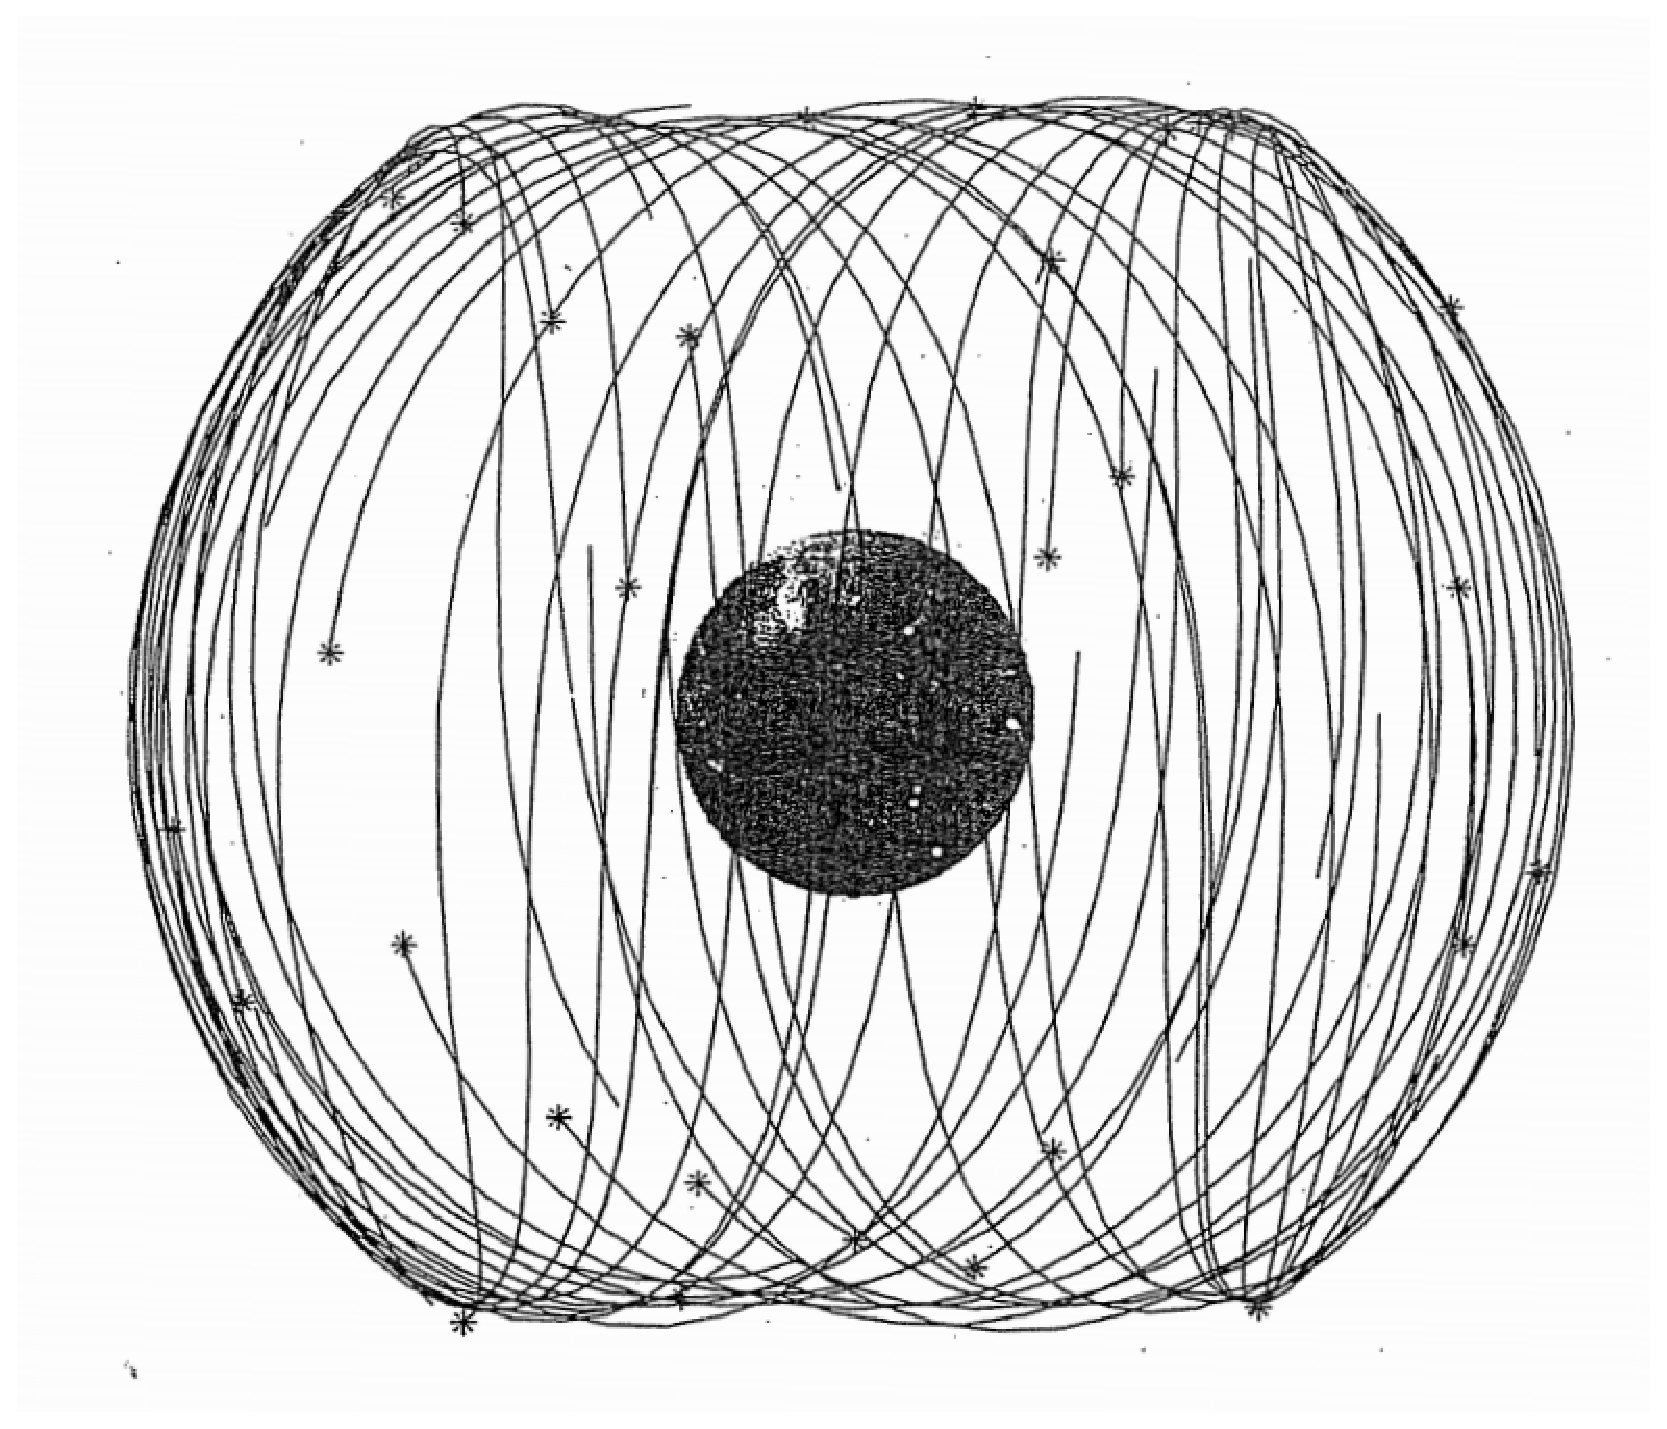
\includegraphics[width=0.4\linewidth]{TeX_files/Part03/chapter09/image/9-2}
		\caption{Satellite orbits as seen in ECEF frame}
		\label{fig:9-2}
	\end{figure}
	Newcomers often have difficulties imagining what the satellite orbits actually look like.Today the constellation consists of some 30 satellites orbiting in six different planes all	making an angle with the Equator of $55^\circ$and rotated $60^\circ$ compared to the previous one.Figure \ref{fig:9-1} is how the situation appears as seen from far away, in what we call an inertial
	frame.
	\begin{figure}
		\centering
		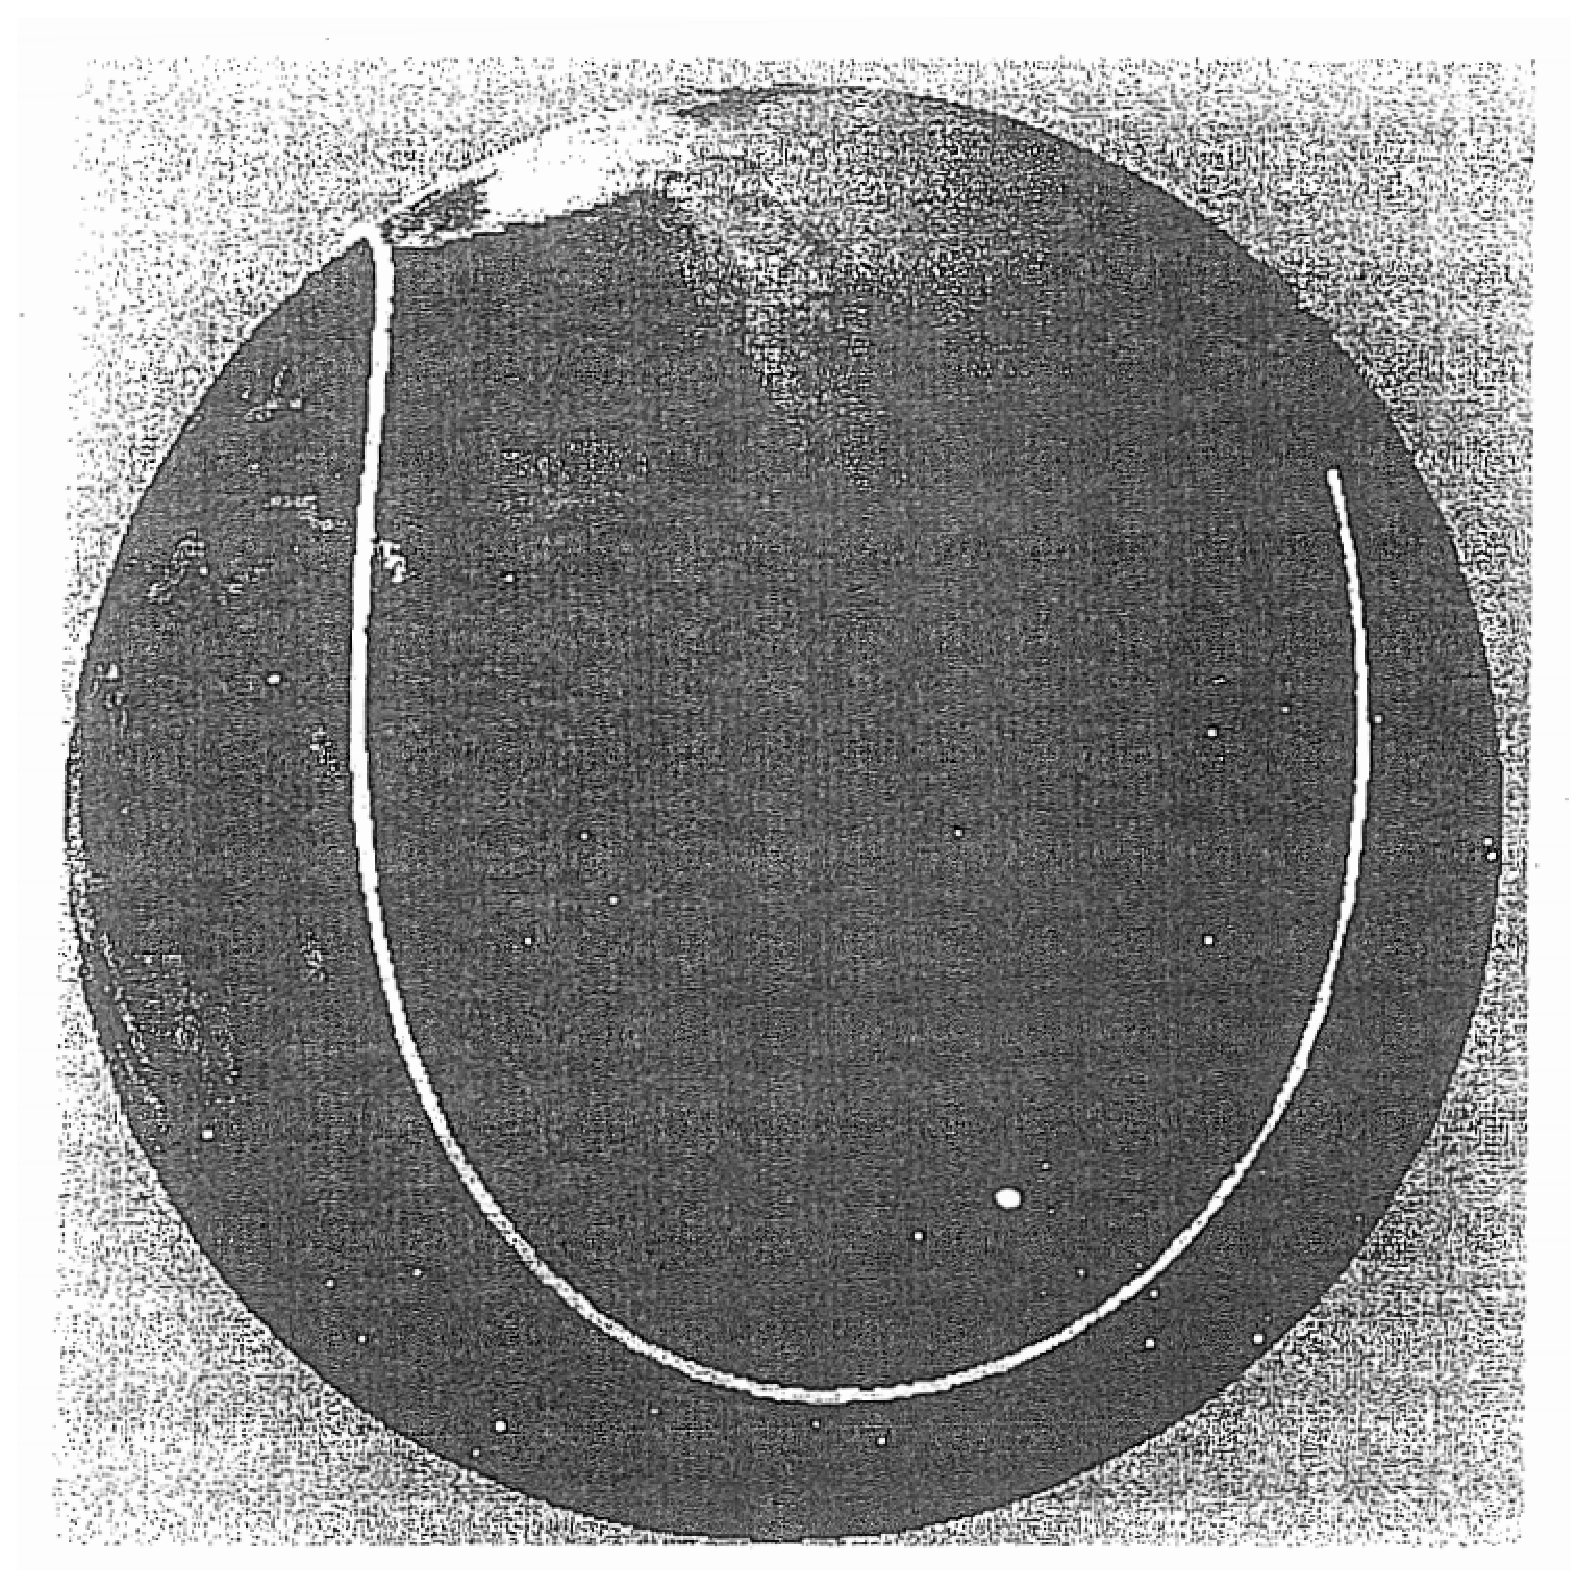
\includegraphics[width=0.4\linewidth]{TeX_files/Part03/chapter09/image/9-3}
		\caption{Sub-satellite points for a selected satellite. The curve is made up of subsatellite points of an arbitrary part of an orbit. The curve is the intersection between the surface of the Earth and the ray from the Earth center to the satellite.}
		\label{fig:9-3}
	\end{figure}
	However, things get less clear if the viewer is on the surface of the rotating Earth. How do the trajectories then look? Very weird. The situation is depicted in Figure \ref{fig:9-2}. Here we use the so-called Earth Centered Earth Fixed coordinate system (ECEF). The ECEF system is in fixed connection with the rotating Earth. That is, a given physical point on the surface maintains its coordinates over time, except for possible movements of the crust.
	
	Finally Figure \ref{fig:9-3} shows a curve made up of the sub-satellite points of an arbitrary part of an orbit. The curve is the intersection between the surface of the Earth and the ray from the Earth center to the satellite. This sub-satellite curve runs within a symmetric belt on both sides of the Equator. It is limited north and south by the inclination angle of the orbit with the Equator.
	